\documentclass[10pt,a4paper]{book}
\usepackage[utf8]{inputenc}
\usepackage{amsmath}
\usepackage{amsfonts}
\usepackage{amssymb}

\usepackage{parskip}

\usepackage{hyperref}

\usepackage{graphicx}
\usepackage{float}
\restylefloat{figure}

\author{Cristian Escudero}
\title{PDS - Resumen}


\begin{document}

\maketitle

\chapter{Introducción a Señales}
\section{Introducción}

Una \textbf{señal} es un fenómeno que representa información. Transporta información sobre el sistema que la produjo, contenida o codificada en un patrón de variaciones de alguna magnitud física. 

Las señales se pueden clasificar de acuerdo a los siguientes criterios:
\begin{itemize}
\item \textbf{Dimensional}: basado en el número de variables indpendientes del modelo de la señal.
\item \textbf{Energético}: si posee o no energía finita.
\item \textbf{Espectral}: basado en la forma de distribución de frecuencias del espectro de la señal.
\item \textbf{Fenomenológico}: basado en el tipo de evolución de la señal, predefinido o aleatorio.
\item \textbf{Morfológico}: basado en el carácter continuo o discreto de la amplitud de la señal o de la variable independiente.
\end{itemize}

\begin{figure}[h!]
  \caption{Clasificación fenomenológica de las señales}
  \label{fig:clasificacion_signals}
  \centering
  \hbox{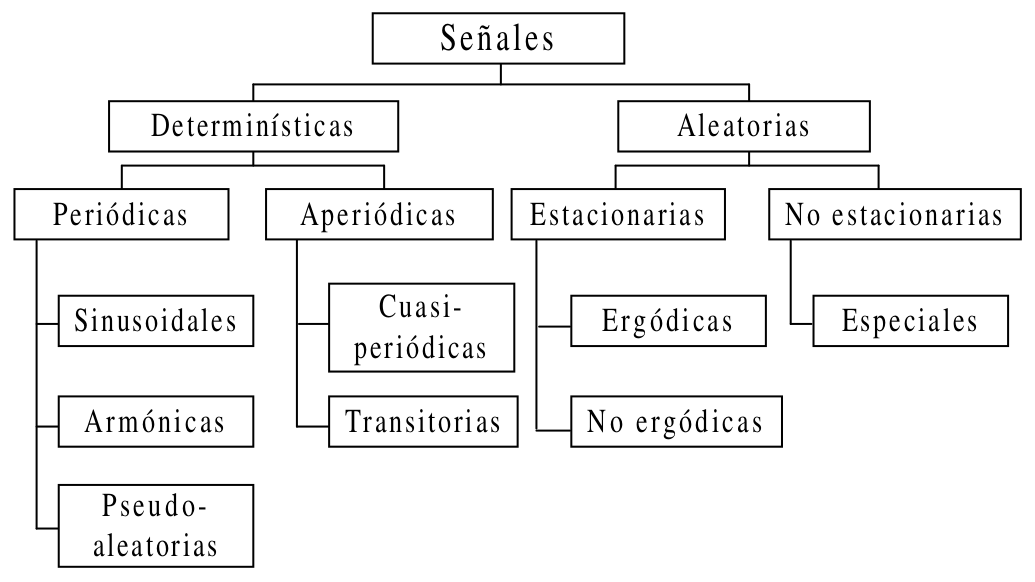
\includegraphics[width=\textwidth-\fboxrule-\fboxrule]{fig1.png}}
\end{figure}

\section{Clasificación de Señales}
\subsection{Clasificación Fenomenológica}

Una señal se puede definir como \textbf{determinística} si sus valores son conocidos de antemano o puede ser predichos exactamente.

Una señal \textbf{continua} es \textbf{periódica} si y sólo si $x(t+T)=x(t) \;\forall \; t\; \epsilon \; (-\infty, \infty)$. Cualquier señal que no es periódica es \textbf{aperiódica}. 

Las señales \textbf{transitorias} son aquellas que agotan su energía en el período de observación.

Las señales \textbf{estocásticas} o \textbf{aleatorias} son aquellas que pueden ser descriptas solamente desde un punto de vista estadístico, ya que existe una cierta \textit{incerteza} acerca de los valores que puede llegar a tomar en cada instante siguiente.

Un proceso aleatorio $\bar{X}(t)$ \textit{estacionario} es aquel en el cual las propiedades estadísticas de la señal no varían con el tiempo. Si, además, las estadísticas a lo largo de una realización cualquiera son iguales a la estadísticas a lo largo de todas las realizaciones, se dice que son \textit{señales aleatorias} del tipo \textbf{ergódica}.

\subsection{Clasificación Morfológica}
Las señales se pueden clasificar según este criterio como:
\begin{itemize}
\item \textbf{Continuas}: la variable independiente es \textbf{continua}.
\item \textbf{Discretas}: la variable independiente es \textbf{discreta}.
\item \textbf{Analógicas}: tanto la amplitud como la variable independiente son \textbf{continuas}.
\item \textbf{Digitales}: tanto la amplitud como la variable independiente son \textbf{discretas}.
\end{itemize}

En términos estrictos, las computadores pueden manejar únicamente señales \textbf{digitales}, ya que las señales \textbf{discretas} pueden ser discretas en el tiempo pero pueden no serlo en amplitud.

Si se \textbf{muestrea} una señal a una velocidad más lenta que la de mayor frecuencia presente en la señal, perderemos información importante, produciendo cambios morfológicos en la señal.

\section{Ruido en señales}
Se denomina \textbf{ruido} a cualquier fenómeno o proceso que perturba la percepción o interpretación de una señal.

Cuando se está en presencia de una señal contaminada con ruido se define una medida de cuánto una señal está contaminada por este, denominada \textbf{relación señal-ruido} (SNR):
\[\xi=\frac{\text{potencia de la señal}}{\text{potencia del ruido}}=\frac{Ps}{Pr}\]
Nota: \textit{Algunos métodos de procesamiento permiten trabajar con pequeñas SNR, gracias a la información de propiedades de la señal conocidas a priori.}

Las \textbf{fuentes de ruido} se pueden clasificar en:
\begin{itemize}
\item \textbf{Externas.} Fuentes de ruido colocadas fuera de cualquier sistema de procesamiento y actuando en él por susceptibilidad.
\begin{itemize}
\item Fuentes de interferencias generadas por artefactos eléctricos.
\item Fuentes de interferencias del tipo electromagnético.
\end{itemize}
\item \textbf{Internas.} Fuentes de ruido dentro del sistema que generan ruido independiente a las condiciones externas.
\begin{itemize}
\item Perturbaciones del tipo impulsivas generadas por la conmutación de corrientes.
\item Ruido de fondo debido a la naturaleza electrónica de los mecanismos de conducción.
\end{itemize}
\end{itemize}

\section{Teoría de la Comunicación}
Se encarga del estudio de los sistemas de comunicación, tanto artificiales como biológicos o naturales. Está compuesta por dos grandes ramas: la \textbf{Teoría de la Señal} y la \textbf{Teoría de la Información y Codificación}.

\subsection{Teoría de la señal}
La \textbf{descripción matemática} de las señales es su objetivo fundamental. Una de sus herramientas básicas y fundamentales es la expansión en términos de \textbf{funciones ortogonales}.

\subsection{Teoría de la información y de la codificación}
Es una \textbf{teoría probabilística} de los mensajes, que tiene en cuenta sus propiedades estadísticas sin importar su significado. Las técnicas de codificación poseen tres objetivos fundamentales:
\begin{itemize}
\item \textbf{Codificación de la fuente:} elimina la redundancia inútil. Incrementa la densidad de la señal. 
\item \textbf{Codificación de canal:} incluye alguna redundancia para permitir posterior detección y corrección de los verdaderos errores. Incrementa la confiabilidad de la señal. 
\item \textbf{Criptografía:} Asegura la privacidad de la comunicación. 
\end{itemize}

\section{Procesamiento de señales}
Es la disciplina técnica que se encarga de la elaboración o interpretación de señales que acarrean información. Uno de sus objetivos principales es la \textbf{extracción} de la \textit{información útil} que se encuentran en la señales.

Para medir una señal, y especialmente una del tipo aleatorio, se trata de estimar el valor de una variable característica, que está vinculada a la misma con un determinado nivel de confianza.

\subsection{Tipos de procesamiento de la señal}
\begin{description}
\item[Análisis.] Trata de aislar las componentes del sistema que tienen una forma compleja para tratar de entender mejor su naturaleza u origen, de encontrar aquellas partes características o \textit{componentes ocultos} que mejor permitan describir la señal, minimizando los efectos del ruido.
\item[Codificación.] Se usa para minimizar los efectos del ruido o reducir la redundancia de una señal.
\item[Detección.] Trata de extraer una señal útil de un ruido de fondo de grandes dimensiones. Las \textit{técnicas de correlación} se usan para detectar la presencia de una señal en un registro determinado.
\item[Filtrado.] Consiste en eliminar o disminuir algunas componentes no deseadas de la señal.
\item[Identificación.] Proceso complementario, que permite clasificar la señal observada. Para establecer las comparaciones se deben "construir" previamente una serie de \textit{plantillas} adecuadas.
\item[Modulación y Traducción.] Formas principales de adaptar una señal a las características de una línea de transmisión, de un filtro analizador, o de un medio de registro.
\item[Regeneración.] Trata de retornar la señal a su forma inicial, después de que ésta haya soportado algun tipo de distorsión.
\item[Síntesis.] Operación opuesta al \textbf{análisis}. Consiste en crear una señal con una forma apropiada mediante la combinación. \textit{Es el problema directo de armar la señal en base a un conjunto de partes.}
\end{description}

\section{Operaciones elementales con señales}
\subsection{Operaciones unarias}
Involucran a una \textbf{única señal}, mientras que las binarias requieren dos señales.
\subsubsection{Operaciones de rango}
Modifican el rango de las señales. Ejemplos: \textit{amplificación}, \textit{rectificación}, \textit{cuantización}. Son definidas como:
\[x_{nuevo}(t)=\rho(x_{viejo}(t))=(p\circ x_{viejo})(t)\]
\subsubsection{Operaciones de dominio}
Modifican la variable independiente. Son definidas como:
\[x_{nuevo}(t)=x_{viejo}(\tau ^{-1} (t))\]
Entre este tipo de operaciones tenemos las que son de la forma:
\[\tau ^{-1} (t)= \alpha t,\]
siendo $\alpha > 1$ (\textit{compresión}), $0<\alpha <1$ (\textit{expansión}), ó $\alpha = -1$ (\textit{reversión}).

La traslación se define como $\tau ^{-1} (t) = t + \theta$, donde $\theta$ es una constante $\mathbb{R}$.

\subsubsection{Muestreo}
Pasa la variable independiente de un dominio \textbf{continuo} a otro \textbf{discreto}. El dominio puede ser discretizado de forma uniforme o no uniforme.

\subsubsection{Interpolación}
Consiste en pasar una señal cuya variable independiente pertenece a un dominio discreto, a una señal cuya variable independiente pertenece a un dominio continuo. Puede ser expreseda como:

\[x(t)=\sum_n x^*(nT)I \left(\frac{t-nT}{T}\right) \]

donde I es la \textbf{función interpolante}.

\subsection{Operaciones binarias}
Se realizan punto a punto entre dos señales (ej: \textit{adición}, \textit{sustracción}, \textit{multiplicación}, \textit{división})

\chapter{Espacios de señales}
\section{Señales, vectores y álgebra lineal}
\subsection{Vectores}
Son colecciones o arreglos de datos que forman una entidad independiente. En forma general, podemos decir que una señal en el espacio N-dimensional es un vector $[x_1,x_2,...,x_N]$, definido como una N-upla ordenada de números. Para estos vectores utilizamos la notación: $\mathbf{x}=[x_n]$, con $n \in \mathbb{N}$, $x_n \in \mathbb{R}$, y $\mathbf{x} \in \mathbb{R}^N$. 

Para señales continuas, la notación es: $\mathbf{x}=[x(t)]$, con $t \in \mathbb{R}$, $x(t) \in \mathbb{R}$, y $\mathbf{x} \in \mathbb{R}^\infty$.

\subsection{Normas}
Provee una medida del tamaño de las señales. La norma de un vector $\mathbf{x}$ es un número $\mathbb{R^+}$ que toma el valor 0 cuando $\mathbf{x}=0$. Cada norma define un tipo especial de medida para un vector. Una norma muy utilizada es la \textit{norma-p}, definida como:
\[
  ||x||_p = \left\{ 
  \begin{array}{l l}
    \left(\sum_{i=1}^N{|x_n|^p} \right)^{1/p}, & \quad 1\leq p <\infty\\
    \text{sup}_{n \in [1,N]}|x_n|, & \quad p=\infty\\
  \end{array} \right.
\]
O para señales continuas:
\[
  ||x||_p = \left\{ 
  \begin{array}{l l}
    \left(\int_{-\infty}^\infty{|x(t)|^p dt} \right)^{1/p}, & \quad 1\leq p <\infty\\
    \text{sup}_{t \in \mathbb{R}}|x(t)|, & \quad p=\infty\\
  \end{array} \right.
\]

\begin{itemize}
\item Si $p=1$, tenemos la norma 1, también conocida como \textit{acción} de la señal.
\item Si $p=2$, tenemos la norma 2. Da una idea del tamaño del objeto en un sentido físico (longitud en vectores).
\subitem $\rightarrow$ La \textit{energía} de una señal está dada como: $E(\mathbf{x})=||\mathbf{x}||_2^2$.
\item Si $p=\infty$, tenemos la norma infinito o \textit{amplitud}: $||\mathbf{x}_\infty||=\text{sup}_{n \in [1,N]}|x_n|$.
\item Cuando la energía de una señal no es finita, es útil definir su \textit{potencia}:
\[P(\mathbf{x})=\text{lím}_{N\rightarrow \infty} \frac{1}{2N}\sum_{n=-N}^N|x_n|^2 \]
\item El \textit{valor cuadrático medio} (RMS) se define como: \textit{RMS}$(\mathbf{x})=\sqrt{P(x)}$.
\item El \textit{valor medio} de una señal queda definido como:
\[m(\mathbf{x})=\text{lím}_{N\rightarrow \infty} \frac{1}{2N}\sum_{n=-N}^N x_n \]
\end{itemize}
\textit{Nota: Para trabajar con señales continuas, se usa lo mismo pero con integrales respecto a t.}

\subsection{Producto interno}
Dado dos vectores $\mathbf{x}, \mathbf{y}\in \mathbb{R}^N$, se define su \textit{producto interno} $\langle\mathbf{x}, \mathbf{y}\rangle \in \mathbb{R}$ como:
\[\langle\mathbf{x}, \mathbf{y}\rangle =\mathbf{x} \cdot \mathbf{y}=x_1 y_1^* + x_2 y_2^* + ... + x_N y_N^*=\sum_{i=1}^N x_i y_i^*\]
dónde el * representa el \textbf{conjugado} en caso de tratarse de valores complejos. El producto interno de un vector consigo mismo es igual al cuadrado de su norma 2.

El producto interno nos da una idea del aporte de una señal en otra. En el caso particular de que la señal sobre la que estamos proyectando tenga norma 2 unitaria, el producto interno es directamente una medida del \textit{parecido}\and entre ambas señales.

\section{Espacios vectoriales y señales}
\subsection{Conjunto de señales}
Consideremos un conjunto de señales $S$. Para determinar si una señal pertenece al conjunto $S$, utilizamos una propiedad o prueba $P$. Un elemento $x$ pertencerá a $S$ si cumple con esta propiedad, es decir: $S={x/P}$.

\subsection{Espacio de señales}
Una señal en particular sólo interesa en relación con las demás señales del conjunto. Para definir una distancia se necesita un funcional $d : {x,y} \rightarrow \mathbb{R}$ que se aplique a todos los pares de elementos del conjunto. Dicho funcional se denomina métrica si cumple las siguientes propiedades:
\begin{enumerate}
\item $d(x,y) \geq 0 \land d(x,y) = 0 \iff x=y,$
\item $d(x,y) =d(y,x)$ (simetría),
\item $d(x,z) \leq 0 d(x,y)+d(y,z)$ (desigualdad del tríangulo).
\end{enumerate}
A un conjunto $S$ al que le hemos asociado una métrica particular $d$ le llamamos espacio métrico. En el caso de que el conjunto $S$ contenga señales, denominamos al par $(S,d)$ \textit{espacio de señales}. Dos métricas diferentes, definidas sobre el mismo conjunto de señales, forman dos espacios de señales \textbf{diferentes}.

\subsection{Espacios vectoriales}
Un \textit{espacio vectorial} $S$ es un cuadruplete $(S,K,+,\cdot)$ que posee:
\begin{itemize}
\item un conjunto de elementos llamados vectores, 
\item un campo de escalares, 
\item una operación de adición, y
\item una operación de producto por un escalar.
\end{itemize}
que satisfacen las siguientes propiedades:
\begin{enumerate}
\item $\mathbf{x}+\mathbf{y}\in S;$ (adición cerrada),
\item $\mathbf{x}+\mathbf{y}=\mathbf{y}+\mathbf{x};$ (adición conmutativa),
\item $\mathbf{x}+(\mathbf{y}+\mathbf{z})=(\mathbf{x}+\mathbf{y})+\mathbf{z};$ (adición asociativa),
\item $\mathbf{x}+0=\mathbf{x};$ ($\exists$ del elemento neutro respecto a la adición),
\item $\alpha \mathbf{x} \in S;$ (producto por escalar cerrado),
\item $\alpha(\beta \mathbf{x})=(\alpha \beta)\mathbf{x};$ (producto por escalar asociativo),
\item $\alpha(\mathbf{x}+\mathbf{y})=\alpha\mathbf{x}+\alpha\mathbf{y};$ (producto escalar distributivo),
\item $1\mathbf{x}=\mathbf{x};$ ($\exists$ del elemento neutro respecto al producto).
\end{enumerate}
Para todo vector que corresponde a $S$, y $\forall \alpha, \beta \in K$.

\subsubsection{Espacios normados}
Dados un espacio vectorial y una definición de norma, se dice que éste es un \textbf{espacio normado} si la norma es finita $\forall$ sus elementos. Lo definimos como: \{$x/||x||_p < +\infty$\}, cuando se trata de señales discretas usamos la notación $l^p(\mathbb{R})$ y cuando las señales son continuas usamos $L^p(\mathbb{R})$. Cada producto interno en un espacio vectorial da lugar a una norma de la siguiente forma: $||x||=\sqrt{\langle\mathbf{x},\mathbf{x}\rangle}$.

Si el espacio es \textit{completo} (asegura continuidad del espacio) con respecto a esta norma, entonces constituye un espacio de \textit{Hilbert}.

\section{Bases y transformaciones}
\subsection{Dependencia lineal y conjuntos generadores}
Dado un conjunto de $N$ vectores $X_0=$\{$\mathbf{x}_i$\}, con $N<\infty$, se dice que este conjunto es \textit{linealmente independiente} si la \textit{combinación lineal}:
\[\sum_{i=1}^N \alpha_i \mathbf{x}_i =0\]
sólo puede satisfacerse siendo nulos todos los escalares $\alpha_i$.

\subsection{Bases}
Dado un espacio vectorial $X$, se dice que el conjunto de vectores $X_0$ constituyen una \textit{base} de $X$ si $X_0$ es \textit{linealmente independiente}, y genera a $X$.

Se llama dimensión $D$ de un espacio vectorial $X$ al \textbf{número} de vectores que tiene una base de dicho espacio.

\subsection{Ortogonalidad y ortonormalidad}
Se dice que un conjunto $X_0$ es \textit{ortogonal} si se verifica que $\forall$ sus elementos:
\[\langle \mathbf{x}_i, \mathbf{x}_j \rangle = 0, \; \forall i \neq j \; 
\land 
\langle \mathbf{x}_i, \mathbf{x}_j \rangle = k, \; \forall i = j \]
dónde $k$ es una constante escalar distinta de cero. En particular, si la constante es $k=1$, se dice que el conjunto es \textit{ortonormal}.

\subsection{Aproximación de señales}
Si se quiere aproximar una señal $\mathbf{y} \in \mathbb{R}$ mediante una combinación lineal de los elementos del conjunto ortogonal $X_0=$\{$x_1,...,x_k,...x_N$\}, necesitamos encontrar los $\alpha_k$ de forma que el \textit{error} entre la señal y la combinación lineal sea mínimo. Se define entonces una forma para medirlo, el \textit{error cuadrático total}:
\[\epsilon=||\mathbf{e}||_2^2=||\mathbf{y}-\hat{\mathbf{y}}||_2^2\]
Para encontrar el mínimo, es necesario hacer $\nabla_\alpha \epsilon=0$ (\textit{ver libro, página 60}).
Podemos calcular $\alpha$ como:
\[\alpha = \frac{\langle \mathbf{v}_1,\mathbf{v}_2 \rangle}{\langle \mathbf{v}_2,\mathbf{v}_2 \rangle}\]

\begin{figure}[h!]
  \caption{Aproximación de vectores utilizando proyecciones. Se puede observar que la mejor manera de calcular $\alpha$ es a través de su proyección ortogonal, minimizando el error en el sentido de la norma euclídea.}
  \label{fig:orto_vectors}
  \centering
  \hbox{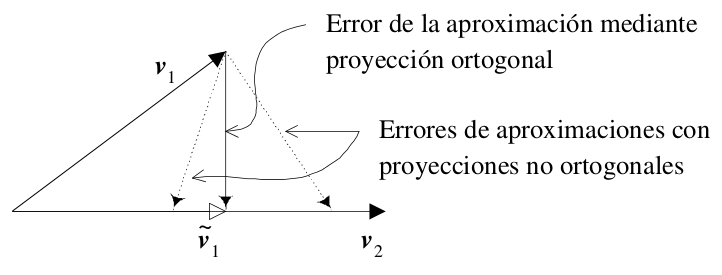
\includegraphics[width=\textwidth-\fboxrule-\fboxrule]{fig2.png}}
\end{figure}

\section{Cambio de base}
Para un espacio vectorial dado existen infinitas bases. Sean $X_0=$\{$x_1,...,x_N$\} y $Y=$\{$y_1,...,y_N$\} dos bases \textit{ordenadas} (una base ordenada es una a la cual ya se le ha establecido un orden) para el mismo espacio vectorial $V$ de dimensión $N$, para cualquier vector $\mathbf{v}$ en $V$ las coordenadas de $\mathbf{v}$ en la base $X_0, \mathbf{v}_{X_0}$, y las coordenadas de $\mathbf{v}$ en la base $Y_0, \mathbf{v}_{Y_0}$, se relacionan por:
\[\mathbf{v}_{X_0}=\mathbf{M v}_{Y_0}\]
\[\mathbf{v}_{Y_0}=\mathbf{M}^{-1} \mathbf{v}_{X_0}\]
donde $\mathbf{M}$ es la matriz no singular de $N \times N$ cuyos elementos están dados por: $\mathbf{y}_i=m_{1i}\mathbf{x}_1 + ... + m_{Ni}\mathbf{x}_N$.

La matriz $\mathbf{M}$ se denomina matriz de \textit{transición} o matriz de \textit{cambio de base} $X_0$ a $Y_0$. Su inversa será la matriz de transición de la base $Y_0$ a la base $X_0$. Un cambio de base no modifica la información presente en la señal, sólo la forma en que ésta es presentada, ya que simplemente se trata de una proyección en términos de otra base.

\paragraph{Relación de Parseval.} La energía se conserva ante un cambio entre base ortonormales:
\[E(\mathbf{x})=\sum_{i=1}^n \alpha_i^2=\sum_{i=1}^n \beta_i^2 k_i\]
dónde $k_i=1$ cuando ambas bases son ortonormales.

\section{Transformaciones lineales}
Una transformación lineal entre dos espacios vectoriales $X$ y $Y$ es una correspondencia que asigna a cada vector $\mathbf{x}$ de $X$ un vector $\mathcal{T}(\mathbf{x})$ en $Y$ de manera tal que: 
\[\mathcal{T}(\alpha_1\mathbf{x}_1+\alpha_2\mathbf{x}_2)=\alpha_1\mathcal{T}(\mathbf{x}_1) + \alpha_2\mathcal{T}(\mathbf{x}_2)\]
para todos los vectores $\mathbf{x}_1$ y $\mathbf{x}_2$ de $X$ y los escaleres $\alpha_1$ y $\alpha_2$.

Los cambios de base son un tipo especial de transformaciones lineales, con características muy interesantes para el procesamiento de señales:
\begin{itemize}
\item son \textbf{uno a uno},
\item son \textbf{invertibles}, y
\item el espacio vectorial $X$ es \textbf{igual} al espacio vectorial $Y$.
\end{itemize}






\chapter*{Licencia}
\begin{center}
Este documento fue escrito en \LaTeX, y editado en \textbf{Texmaker}.

Basado en el libro \textbf{Introducción a las Señales y los Sistemas Discretos} de Milone, Rufiner, Acevado, Di Persia y Torres.
\vfill

\href{http://creativecommons.org/licenses/by-sa/3.0/}{

\includegraphics{CC.png}}

Este obra está bajo una \href{http://creativecommons.org/licenses/by-sa/3.0/}{licencia Creative Commons Atribución-CompartirIgual 3.0 Unported}
\end{center}
\end{document}